% Prácticas de Estadística para el GII de la UGR, una aproximación con Python
% José David Rico Días
% Bajo Licencia Creative Commons 4.0 (BY-NC-SA)


% CONSIDERACIONES SI NO USAS OVERLEAF   %
% Compilación : XeLaTex                 %
% Lista de paquetes:                    %
%   -   fontspec                        %
%   -   hyperref                        %
%   -   grapchicx                       %
%   -   geometry                        %
%   -   babel                           %
%   -   listings                        %
%   -   xcolor                          %
%   -   float                           %


% Configuración de la clase book %
%------------------------------------------------------------------------------%

% FAQ %
%       Quiero cambiar el color de la página y del texto        %
%       ---     Busca con CTRL-F el comando '\pagecolor'. Puedes cambiar el color al que más te apetezca, o comentar los comandos '\color' y '\pagecolor' para que aparezca la opción por defecto. Recuerda que el logo de la UGR está en color blanco, puesto que por defecto está configurada la versión de ordenador.


\documentclass[openany,a4paper]{book}

% Indenta con números hasta 4 %
\setcounter{secnumdepth}{3}
\setcounter{tocdepth}{2}

\setlength{\parindent}{0em}
\setlength{\parskip}{0.1236cm} % 2*(1/phi) %

% Paquetes %
%------------------------------------------------------------------------------%

% Uso de fuentes especiales %
\usepackage{fontspec}
% Configuración de la fuente % Se usa la fuente San Francisco; la que usa Apple %
\setmainfont[
Path=./fonts/,      % Directorio de las fuentes %
BoldFont=SF-Bold.otf,
ItalicFont=SF-Italic.otf,
BoldItalicFont=SF-Bold-Italic.otf
]{SF.otf}

% Permite hipervínculos en el PDF, lo que facilita la navegación %
\usepackage[breaklinks=true,hidelinks]{hyperref}

% Gráficos % Insertar imágenes %
\usepackage{graphicx}

% Ajuste de márgenes. Optimizado para lectura en ordenador %
\usepackage[lmargin=2cm,rmargin=2cm,top=2cm,bottom=2cm,headsep=3mm]{geometry}
% Con esta configuración conseguimos que el PDF se pueda leer en un e-book. %
% Puede que no sea una feature muy interesante.                             %
%
%       \usepackage[papersize={95mm,125mm},lmargin=1.5mm,rmargin=1.5mm,top=7mm,bottom=1.5mm,headsep=3mm]{geometry}

% Idioma %
\usepackage[spanish]{babel}

% Introducir código de python %
\usepackage{listings} 
\usepackage[usenames]{xcolor}
 
\definecolor{codegreen}{rgb}{0,1,0}
\definecolor{codegray}{rgb}{0.5,0.5,0.5}
\definecolor{codepurple}{rgb}{0.78,0,1}

% Definicion de colores de fondo y texto %
\pagecolor{black}
\color{white}


\lstdefinestyle{mystyle}{
    backgroundcolor=\color{black},   
    commentstyle=\color{codegreen},
    keywordstyle=\color{magenta},
    numberstyle=\tiny\color{codegray},
    stringstyle=\color{codepurple},
    basicstyle=\ttfamily\footnotesize,
    breakatwhitespace=false,         
    breaklines=true,                 
    captionpos=b,                    
    keepspaces=true,                 
    numbers=left,                    
    numbersep=3pt,                  
    showspaces=false,                
    showstringspaces=false,
    showtabs=false,                  
    tabsize=1
}

\lstset{style=mystyle}

% Posicion de figuras %
\usepackage{float}

% Rodear figuras con texto %
\usepackage{wrapfig}

\usepackage{float}

% Comandos propios %
%------------------------------------------------------------------------------%

% Script para la creación de citas a un personaje %
\newcommand{\chapquote}[3]{\begin{quotation} \textit{#1} \end{quotation} \begin{flushright} - #2, \textit{#3}\end{flushright} } 

%------------------------------------------------------------------------------%

\begin{document}
 
\begin{titlepage}
	\begin{center}		
		\vspace*{1.0cm}
		\begin{Huge}
			\textbf{Prácticas de estadística para el GII UGR, una aproximación con Python}\\
		\end{Huge}	
		\vspace*{1.0cm}
		\rule{150mm}{0.1mm}\\
		
		\vspace*{1.5cm}
		\begin{figure}[htb]
			\begin{center}
				
\includegraphics[width=9cm]{images/logotypes/Logo UGR.png}
			\end{center}
		\end{figure}
        \huge{José David Rico Días}\\
		\vspace*{1cm}
	    \Large{\today}
	\end{center}		
\end{titlepage}

\thispagestyle{empty}

Este documento está bajo la licencia CC BY-NC-SA. Junto a este documento debes haber recibido una copia de la licencia correspondiente. Si no es así puedes consultar la licencia en el siguiente enlace: 

\textbf{\href{https://creativecommons.org/licenses/by-nc-sa/4.0/legalcode.es}{https://creativecommons.org/licenses/by-nc-sa/4.0/legalcode.es}}

This document is under the CC BY-NC-SA license. Among this document you may have received a license's copy. If not, you can read the license in the following link: 

\textbf{\href{https://creativecommons.org/licenses/by-nc-sa/4.0/legalcode.en}{https://creativecommons.org/licenses/by-nc-sa/4.0/legalcode.en}}

\newpage

\thispagestyle{empty}

\vspace*{9cm}
\chapquote{"Python is an experiment in how much freedom programmers need. Too much freedom and nobody can read another's code; too little an expressiveness is endangered."}{Guido von Rossum}{Creador de Python}


\chapter*{Motivación}

\thispagestyle{empty}

Durante el inicio del del 2º cuatrimestre, empecé las prácticas de Estadística. Comenzamos aprendiendo el lenguaje de programación R, concretamente R Commander. Yo que ya conocía Python y las famosas bibliotecas SciPy y NumPy, pensé que con la versatilidad que ofrece este maravilloso lenguaje, sería más adecuado para un Ingeniero Informático.

\chapter*{Sobre este manual}

\thispagestyle{empty}

ESTE NO ES UN MANUAL O TUTORIAL DE PYTHON, si lo que buscas es una introducción a Python, te recomendaré miles de cursos y libros, pero este manual no es para ti. A los puristas del lenguaje debo decirles que sí, se puede aprender a usar las librerías NumPy, ScyPy, Pandas... Sin saber de tuplas, diccionarios, herencia, etc.


Si te has quedado, es recomendable que trabajes con este manual en PDF en el ordenador. Está compilado en fondo negro para que no se te canse la vista al leer con la pantalla.

Además, puedes consultar el GitHub con todos los datos y las soluciones a los ejercicios en el siguiente enlace \textbf{\href{https://github.com/davidricodias/Practicum_ES_GII_UGR_Python}{https://github.com/davidricodias/Practicum\_ES\_GII\_UGR\_Python}}.

\tableofcontents
\thispagestyle{empty}

\newpage

\chapter{Introducción}

\setcounter{page}{1}

\section{¿Qué es Python?}

Python es una lenguaje de \textit{scripting}; no crea un ejecutable, sino que las órdenes se interpretan línea a línea. A día de hoy lo usan empresas como Google, Facebook, Amazon, ... 

El ranking PYPL (basado en las búsquedas de Google) sitúa a Python en el primer puesto \footnote{\textbf{\href{http://pypl.github.io/PYPL.html}{http://pypl.github.io/PYPL.html}}}. El ranking de IEEE Spectrum (La revista de informática de la IEEE) lo sitúa en primer puesto \footnote{\textbf{\href{https://spectrum.ieee.org/computing/software/the-top-programming-languages-2019}{https://spectrum.ieee.org/computing/software/the-top-programming-languages-2019}}}, entre otros...

Durante este curso, conocerás las bases (orientadas a la estadística) de un lenguaje actual, altamente demandado y muy fácil de aprender.

\section{Nuestro entorno de trabajo}

Para las prácticas usaremos el entorno \textbf{Jupyter}. Es ampliamente usado en \textit{Data Science}, \textit{Machine Learning}, cálculo científico, etc.

\begin{figure}[H]
    \centering
    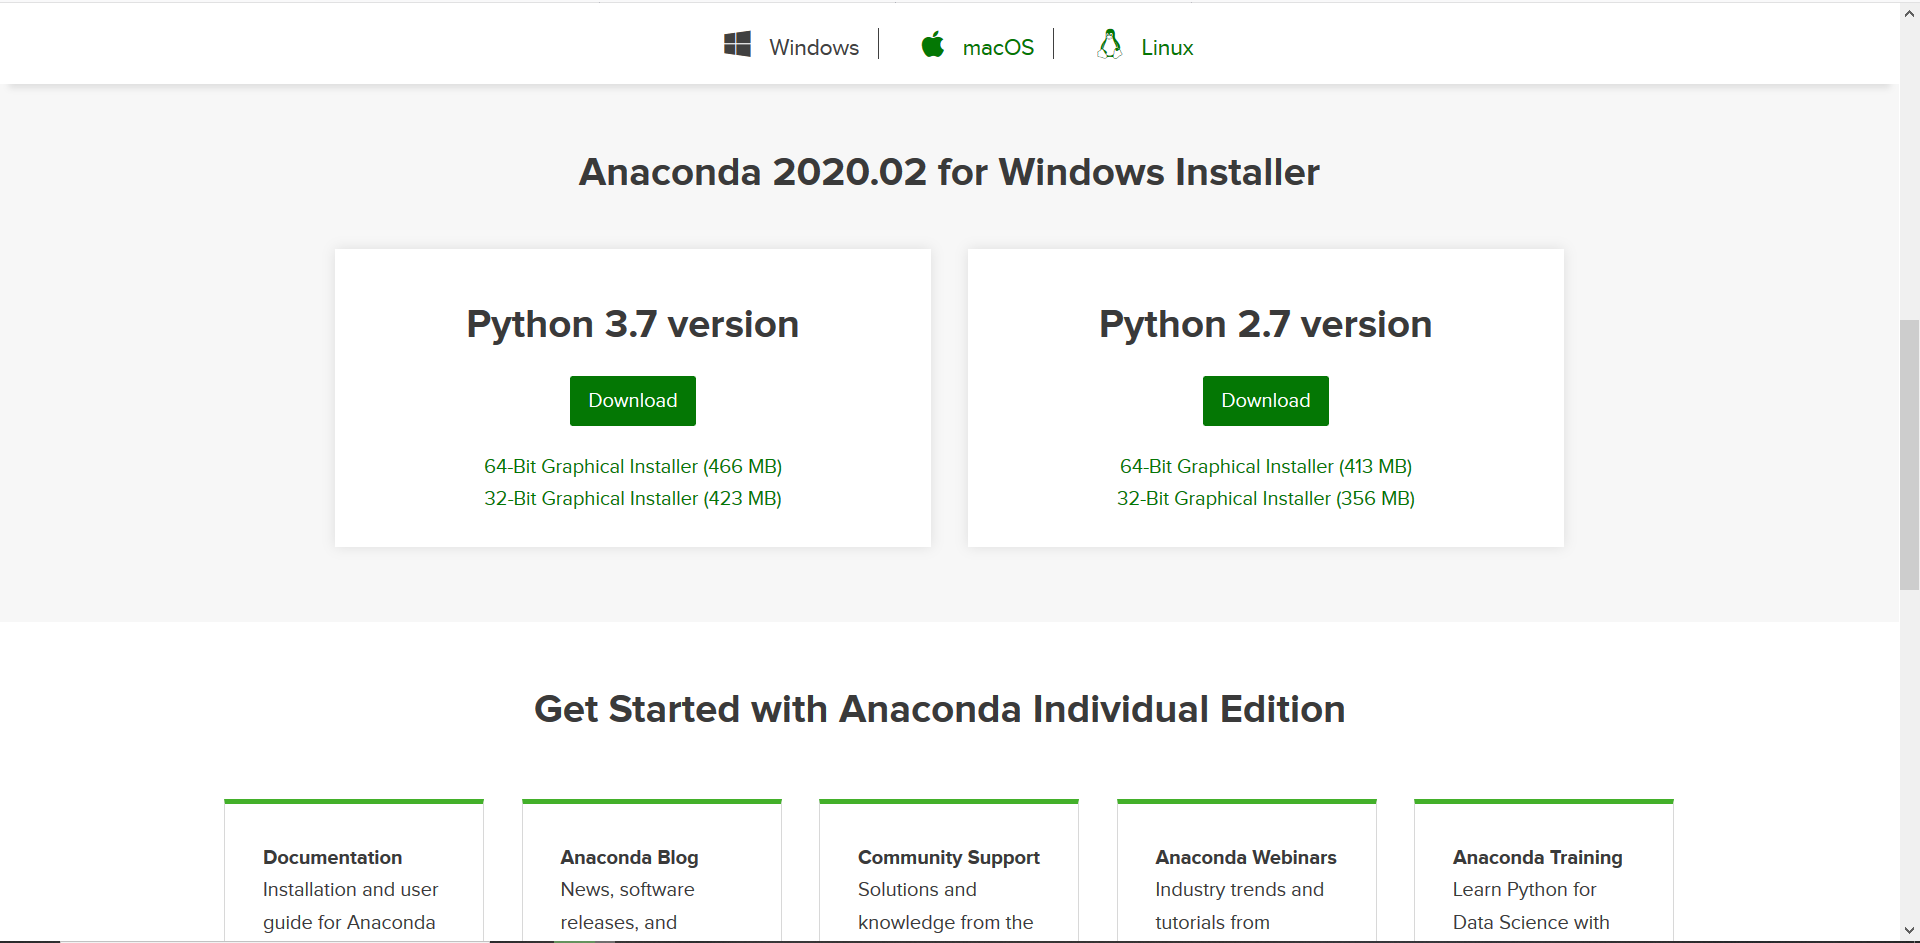
\includegraphics[width=0.618\linewidth]{images/screenshots/anaconda/anaconda_download.PNG}
    \caption{Instalación de Anaconda}
\end{figure}

Para la instalación nos descargaremos el entorno Anaconda en \href{https://www.anaconda.com/distribution/#download-section}{este link}\footnote{\href{https://www.anaconda.com/distribution/\#download-section}{https://www.anaconda.com/distribution/\#download-section}}. Escogemos la versión 3.7, pero si estás leyendo esto y no está exactamente la versión 3.7, escoge la versión que empiece por 3.

\begin{figure}[H]
    \centering
    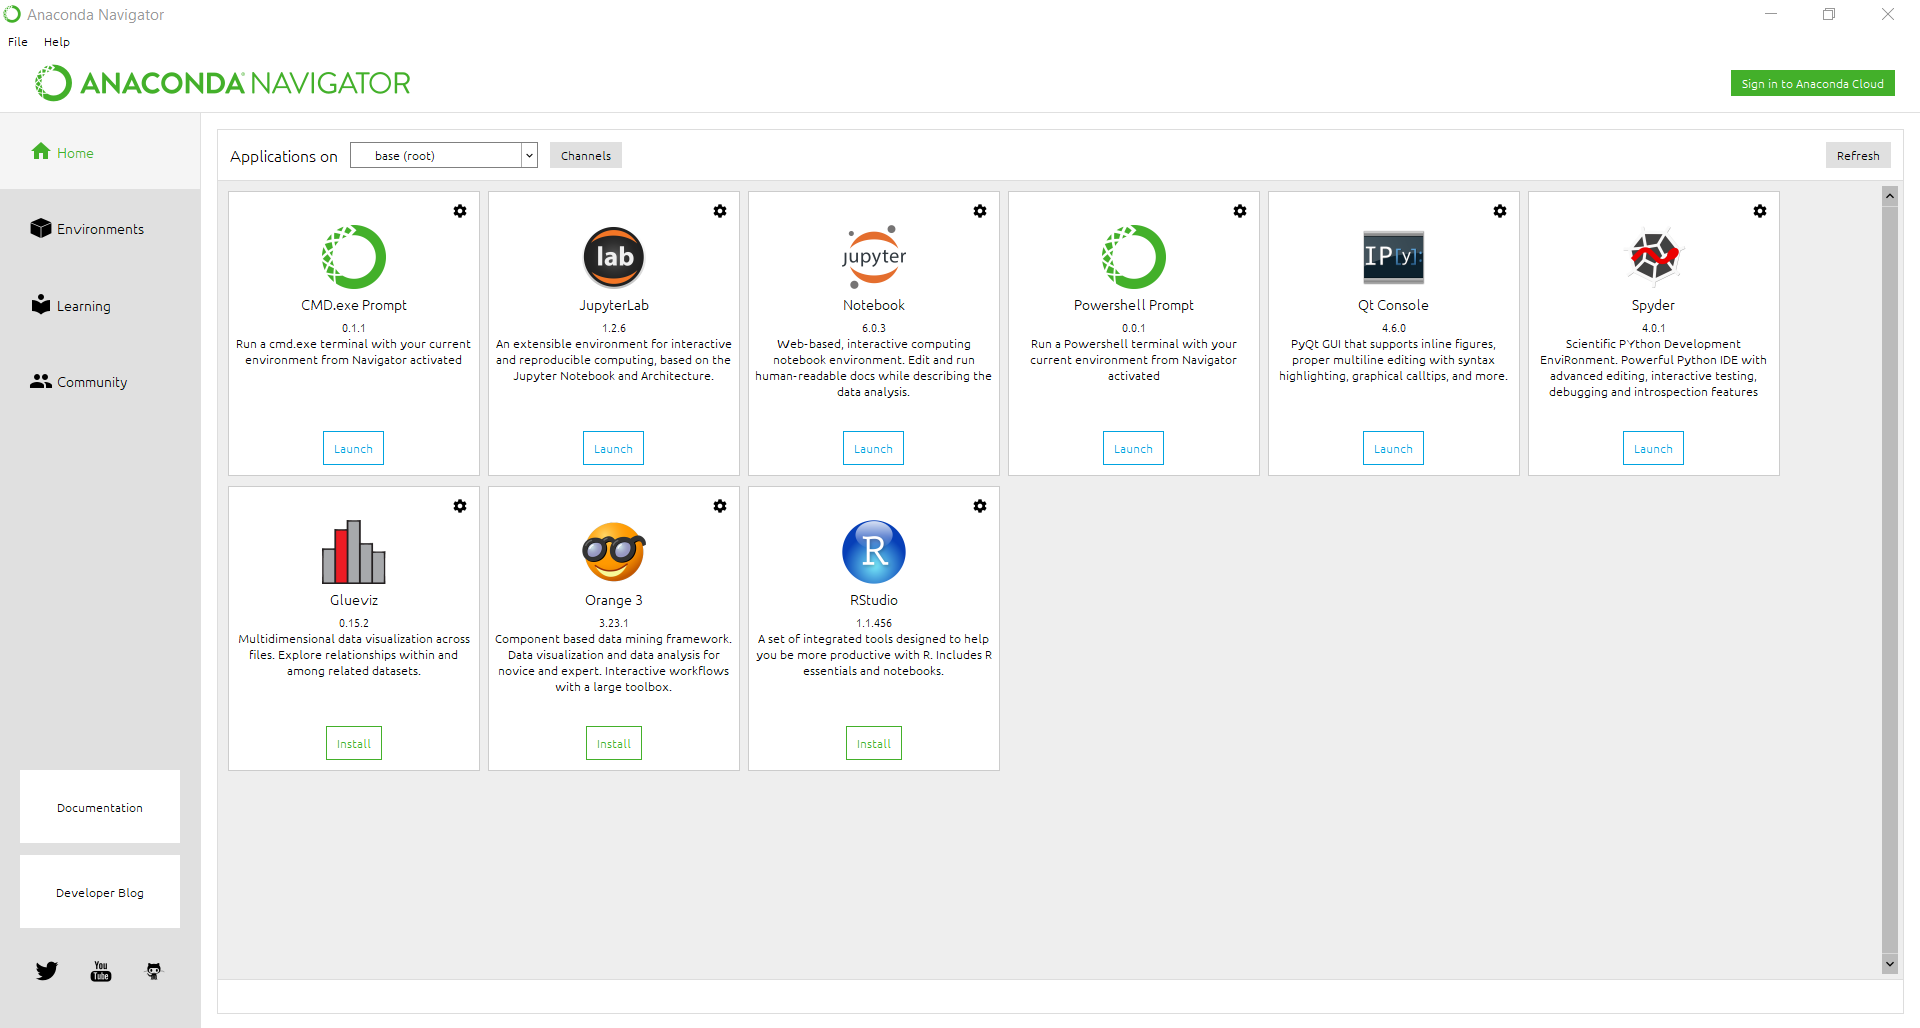
\includegraphics[width=0.618\linewidth]{images/screenshots/anaconda/anaconda_in.png}
    \caption{Entornos disponibles en Anaconda}
\end{figure}

Iniciamos \texttt{Anaconda Navigator} en las aplicaciones de nuestro PC, y a continuación un cuaderno Jupyter (o \textit{Jupyter Notebook}.

Tras esto debe abrirse una pestaña en nuestro navegador predeterminado.

\begin{figure}[H]
    \centering
    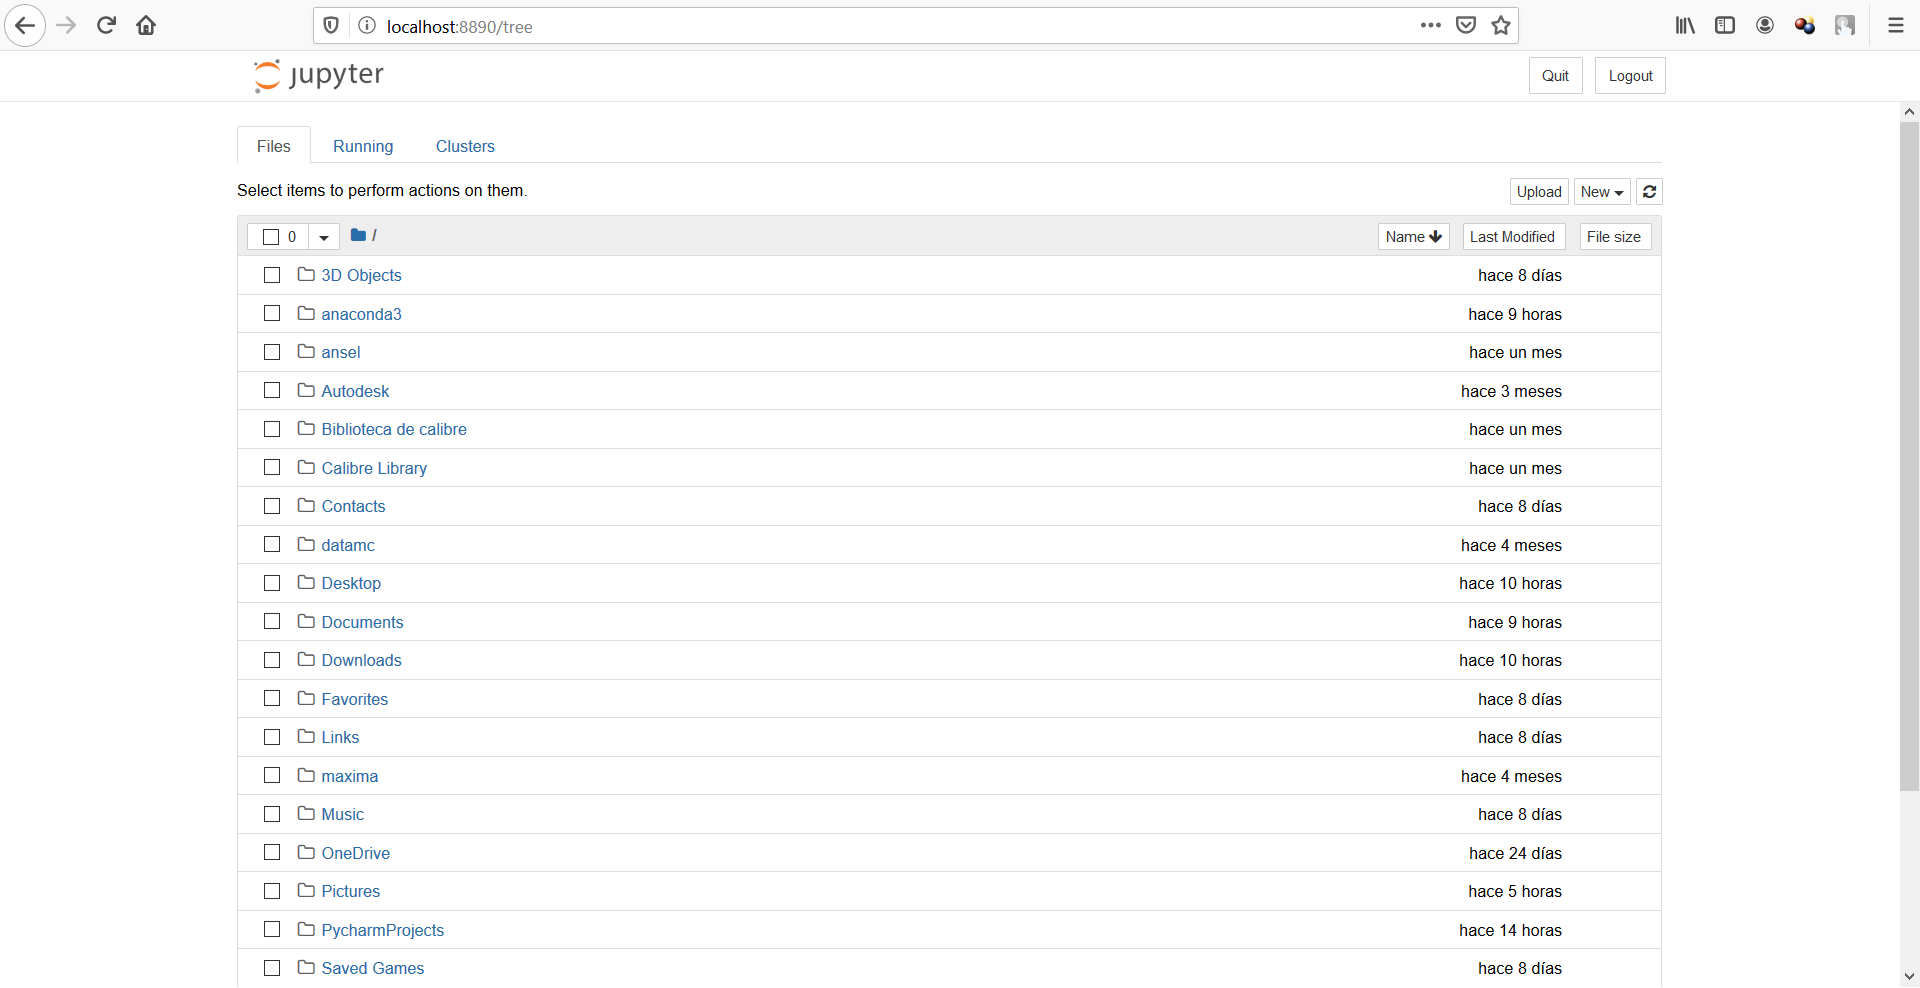
\includegraphics[width=0.618\linewidth]{images/screenshots/jupyter/jupyter_init.png}
    \caption{Entorno Jupyter}
\end{figure}

Te recomiendo crear una carpeta donde trabajes exclusivamente los ejercicios y ejemplos del manual. Puedes hacerlo desde Jupyter con \texttt{New->Folder}. Además deberías descargar los ejercicios que vamos a trabajar en este enlace:

\begin{figure}[H]
    \centering
    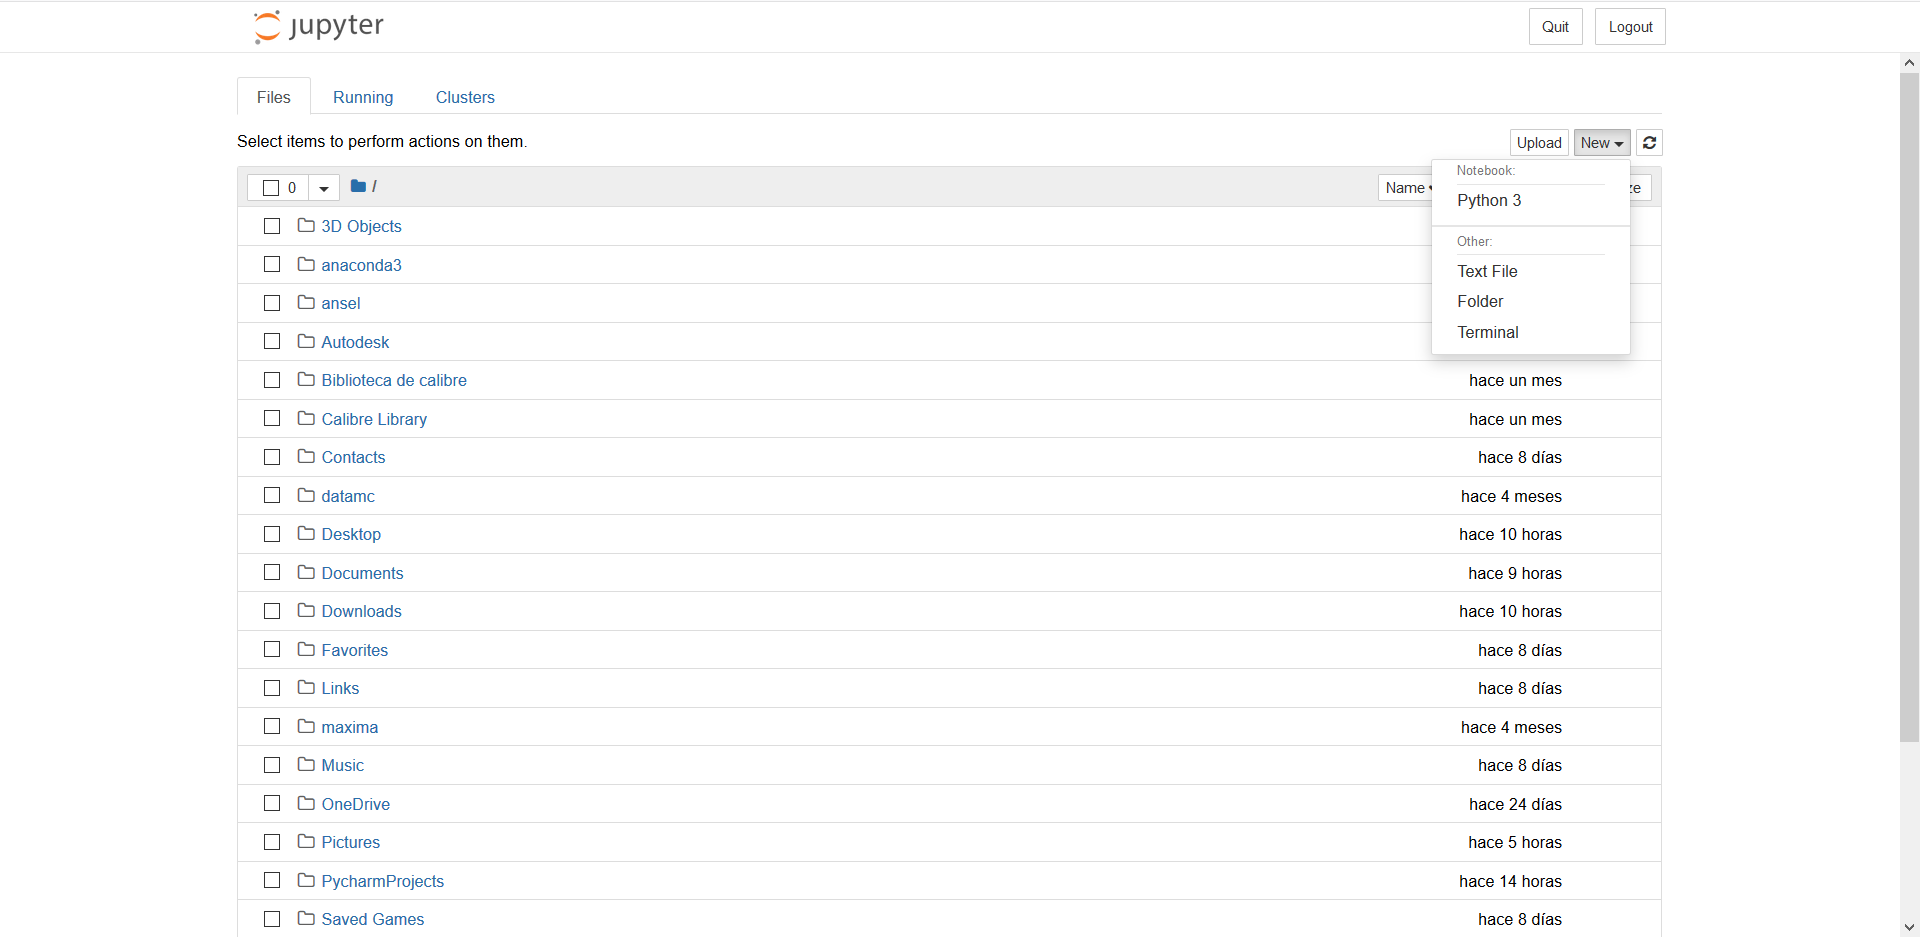
\includegraphics[width=0.618\linewidth]{images/screenshots/jupyter/jupyter_init_new_folder.png}
    \caption{Cómo crear un directorio desde Jupyter}
\end{figure}

Y con esto ya puedes empezar a \textit{trastear} con el entorno Jupyter (o \textit{Jupyter enviroment}).

Si eres una persona que necesita usar LaTex para sus trabajos o investigaciones esto te interesa: JuPyter te permite exportar todo el notebook a LaTex usando XeLaTex como compilador. Además soporta lenguaje LaTex dentro del propio Notebook, lo que significa que puedes hacer cualquier tipo de trabajo usando solo Jupyter...

\section{Calentamiento}

Antes de siquiera calcular una media, debemos familiarizarnos un poco con Python. Empezaremos creando un archivo nuevo y saludando con \texttt{"¡Hola mundo!"}.

Para ello ve a la carpeta donde trabajes y selecciona \texttt{New->Python 3}. Esto debería abrir un \textit{notebook} de Jupyter.

\begin{figure}[H]
    \centering
    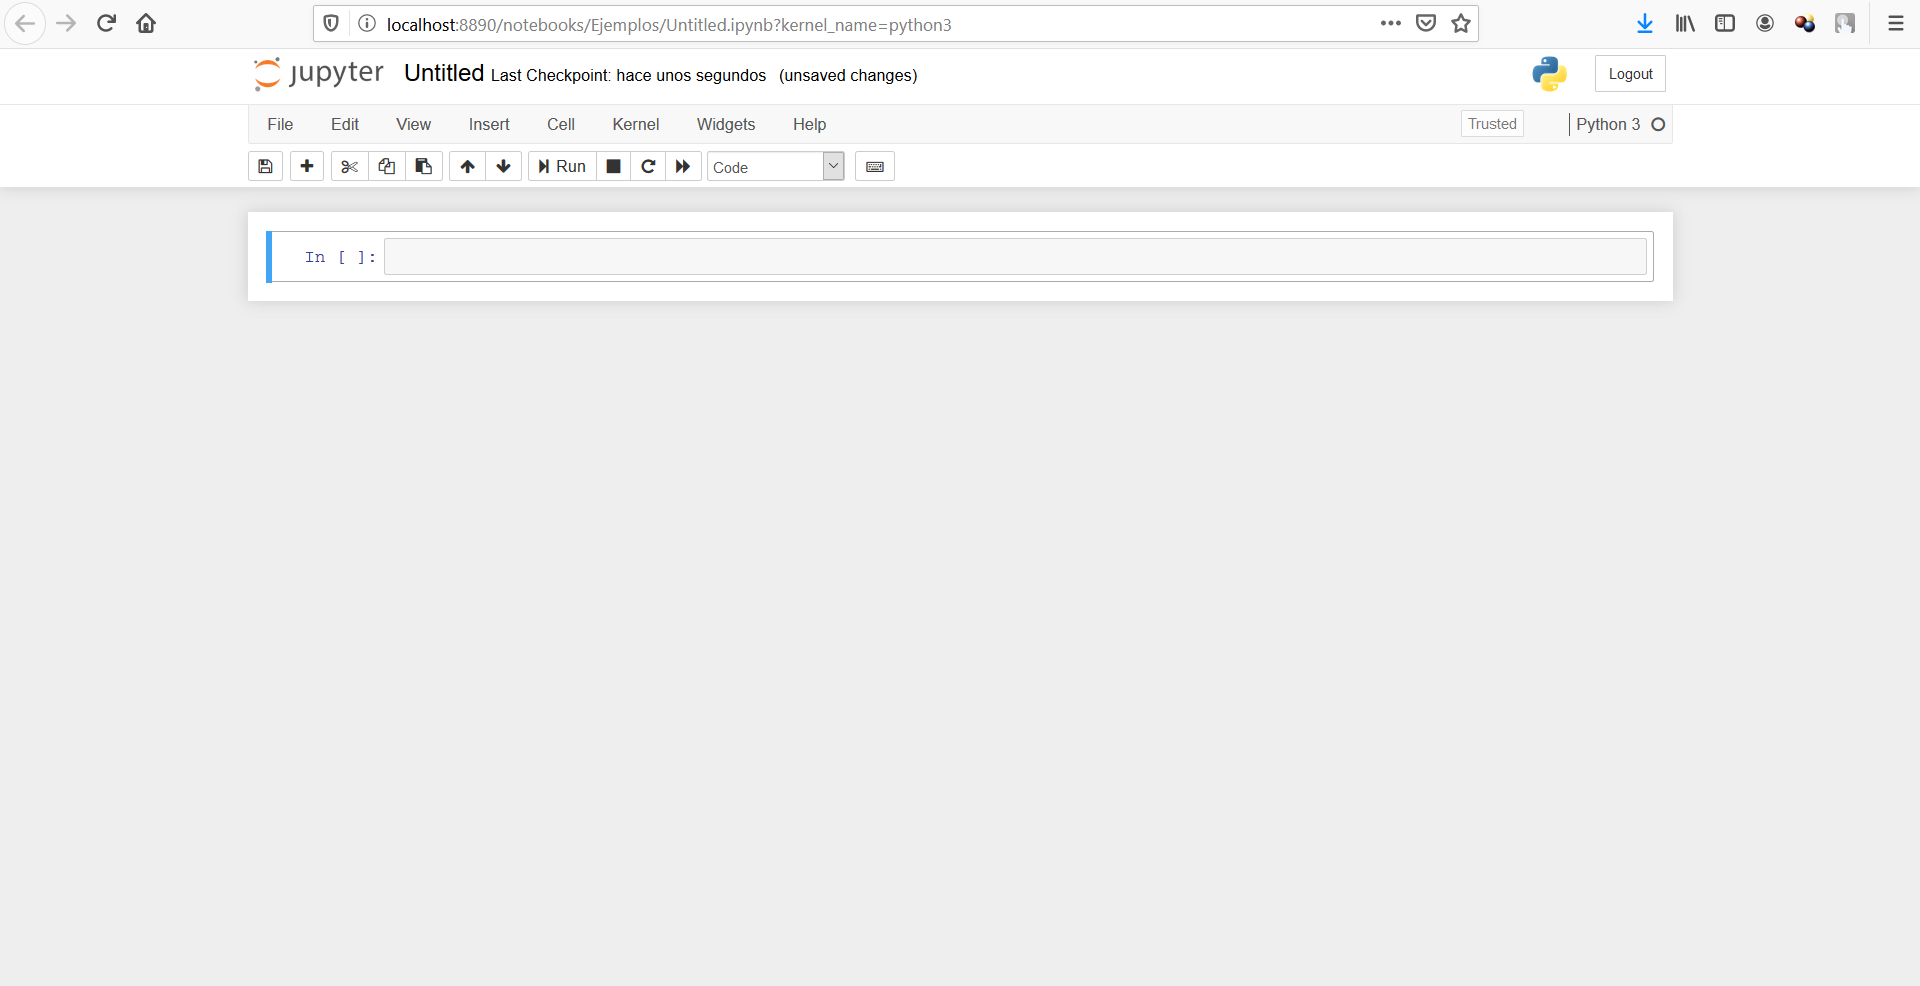
\includegraphics[width=0.618\linewidth]{images/screenshots/jupyter/jupyter_init_notebook.png}
    \caption{Tu primer notebook de Jupyter}
\end{figure}

Escribe en el recuadro el siguiente código:
\begin{lstlisting}[language=Python]
    print("¡Hola mundo!")
\end{lstlisting}{}

Y presiona \texttt{Shift+Enter}.

Nota como no hay que incluir bibliotecas, ni crear un main, ...

\textbf{Antes de empezar recuerda que todo el código está hecho en notebook y subido a github para que no tengas que escribir}

\subsection{Lo básico}

Para usar este manual no hace falta saber programar Python, pero sí se espera que sepas algo de programación, por lo que solo daré una pasada general y me centraré en lo que más usaremos.

\subsubsection{Indentación}

Python es un lenguaje sensible a la indentación, eso quiere decir que al escribir funciones o clases se deben respetar las indentaciones para saber lo que está dentro y lo que está fuera de la función/clase.

Esto obliga a mantener un estilo de codificación más limpio.

\subsubsection{Errores}
Cuando ocurra un error durante la interpretación del código, Python lanzará un \textit{Traceback} o traza. No suelen ser muy explicativas, pero sí señalan la línea donde se ha producido.

\subsubsection{Variables}

La principal característica es que no es necesario declarar el tipo de variable que queremos usar.

\begin{lstlisting}[language=Python]
    a=5
    b="Hola"
    c=a*10
    print(b,c)
\end{lstlisting}

Python automáticamente asigna el tipo de dato que considera más conveniente.

\subsubsection{Listas}

Funcionan igual que los vectores de C, excepto porque pueden guardar \textit{cualquier} tipo de dato, incluso mezclado.

Para crear una lista fácilmente podemos usar la función \texttt{range()}:
\begin{lstlisting}[language=Python]
    a=range(10)
    print(a)
\end{lstlisting}

Habrás notado que al imprimir \texttt{a}, nos dice que es un rango de 0 a 10, lo cual es cierto, pero no es la clase de salida que esperamos de una lista. Prueba ahora con la función \texttt{list()}:

\begin{lstlisting}[language=Python]
    a=range(10)
    print(list(a))
\end{lstlisting}

Y ahí está, tu primera lista en Python.

\subsubsection{Condicional \texttt{if-elif-else}}

Como en C, se introduce una expresión booleana y si devuelve verdadero se accede al bloque de instrucciones.

\begin{lstlisting}[language=Python]
    if 1==1 :
        # Este bloque se va a ejecutar
        print("Este bloque")
        print("se va a ejecutar")
    elif 2>3 :
        print("Esto es imposible")
    else :
        print("Esto es un else")
\end{lstlisting}

Aquí hay mucho que extraer:
\begin{itemize}
    \item Hay un tipo de bloque que no existe en C, \texttt{elif}. Este equivale a escribir \texttt{else if}.
    \item Los bloques \texttt{if} y \texttt{elif} no necesitan paréntesis y terminan en "\texttt{:}".
    \item Los comentarios se escriben poniendo \texttt{\#}.
\end{itemize}


\subsubsection{Bucle \texttt{for}}

Los siguientes códigos son equivalentes (en C++ y Python):

En C++ :
\begin{lstlisting}[language=C++]
    #include <iostream>
    
    using namespace std ;
    
    int main() {
        for( int i=0 ; i<10 ; i++ ) {
            cout << i << endl ;
        }
        return 0 ;
    }
\end{lstlisting}

Y en Python :

\begin{lstlisting}[language=Python]
    for i in range(10) :
        print(i)
\end{lstlisting}

La principal característica del bucle \texttt{for} en Python es poder iterar una variable sobre cualquier conjunto de datos. En este caso ha sido sobre una lista, pero podría ser sobre nombres de un archivo, conexiones a otros ordenadores, objetos...

\subsubsection{Bucle \texttt{while}}

Mientras se cumpla la condición, se ejecuta el bloque:
\begin{lstlisting}[language=Python]
    var = 0
    while 0 < 10:
        print("Hola")
        var +=1
\end{lstlisting}

Debes notar 2 cosas: la palabra \texttt{True} se ha coloreado, ya que \texttt{True} y \texttt{False} son palabras reservadas en Python; siempre se escriben con la primera letra en mayúscula. Lo segundo es que la variable \texttt{var} va aumentando de 1 en 1, pero no he escrito \texttt{var++}; la expresión \texttt{++} no existe en Python.

\subsubsection{Funciones}

Para crear una función, escribimos la palabra reservada \texttt{def} seguida del nombre de la función, los parámetros y "\texttt{:}". Con un ejemplo será más claro:

\begin{lstlisting}[language=Python]
    def diHola( nombre ) :
        print("Hola",nombre)
    
    diHola("Pepito")
\end{lstlisting}

Una característica muy interesante es que podemos definir y usar funciones dentro de funciones.

\section*{Funciones usadas en este capítulo}

\begin{table}[H]
\centering
\begin{tabular}{lll}
print() & range() & list()
\end{tabular}
\end{table}

\chapter{Manos a la obra}

\section{Hola media}

\section{Mediana}

\section*{Funciones usadas en este capítulo}

\chapter{Un poco de color}

\section*{Funciones usadas en este capítulo}

\end{document}